\chapter{FreeRTOS redundancy API} % Grammarly OK
\label{freertos_modification}

\section{Timed tasks addition}

\subsection{Introduction}

Atop of all FreeRTOS functionality ability to measure task's run time and its total time (running + other states) is not provided. Such feature is extremely useful for hard real-time embedded systems. In such systems breaching the deadline means the failure of the system.

Adding the aforementioned timers to the tasks means the ability to detect if the task ran for too long or it didn't get enough processor time. When such an event has occurred it can be properly handled. For example, for an embedded system that is periodically polling the speed of rotation of an engine if it isn't polled in time, it can raise an alarm to force the reading. \autoref{appendix_cmd_ref_freertos} contains the command reference for the timed tasks.

\subsection{Architecture}


When timed tasks are created two software timers are created tied to it. One is called overrun timer and is used to detect when the task executes for longer than allocated. Second, the overflow timer is used to detect if the task is running properly asynchronously i.e. timer doesn't stop ticking even if the timed task is inactive.  

The overflow timer is started when the timed task is switched to the first time. It is started from the context switch. Code section is shown in \autoref{fig:freertos_overflow_start}. Function \code{prvStartOverflowTimer} checks if the timer is started and if it is not it starts the timer otherwise it does not do anything.


\begin{figure}[H]
\begin{changemargin}{1cm}{1cm}
\begin{lstlisting}[escapeinside={(*}{*)}, numbers=left, numberstyle=\tiny, stepnumber=1, language=c]
/* Check for stack overflow, if configured. */
taskCHECK_FOR_STACK_OVERFLOW();

/* Select a new task to run using either the generic C or port
   optimised asm code. */
taskSELECT_HIGHEST_PRIORITY_TASK();


#if( INCLUDE_xTaskCreateTimed == 1 )
{
   BaseType_t xHigherPriorityTaskWoken = pdFALSE;

   prvStartOverflowTimer( pxCurrentTCB, xIsSwitchContextFromISR, &xHigherPriorityTaskWoken );

   if(xHigherPriorityTaskWoken != pdFALSE)
   {
        /* Select a new task to run using either the generic C or port
           optimised asm code.
           Highest priority should be the timer daemon. */
        taskSELECT_HIGHEST_PRIORITY_TASK();
   }
}
#endif /* INCLUDE_xTaskCreateTimed == 1 */
\end{lstlisting}  
\end{changemargin}
\caption{Starting of the overflow timer from the file task.c}
\label{fig:freertos_overflow_start}
\end{figure}

The overrun timer is only a variable in the task control block. It is incremented every tick while the timed task is running. When the overrun timer is about to expire (1 tick before) a software timer is started. Next tick, the software timer triggers the overrun callback. Code for incrementing (\autoref{fig:freertos_overrun_increment}) is called from the function xTaskIncrementTick which itself is called from the tick interrupt. Overrun timer (of period 1 tick) is started from the context switch function, with code shown in \autoref{fig:freertos_overrun_start}.

\begin{figure}[H]
\begin{changemargin}{1cm}{1cm}
\begin{lstlisting}[escapeinside={(*}{*)}, numbers=left, numberstyle=\tiny, stepnumber=1, language=c]
#if INCLUDE_xTaskCreateTimed == 1
    BaseType_t prvIncrementOverrunTick(void)
    {
        BaseType_t xReturn = pdFALSE;
        if( pxCurrentTCB->xOverrunTimer != NULL )
        {
            pxCurrentTCB->xOverrunTicks++;
            if(pxCurrentTCB->xOverrunTicks >= ( pxCurrentTCB->xOverrunTicksMax - 1 ) )
            {
                xReturn = pdTRUE;
            }
        }
        return xReturn;
    }
#endif
\end{lstlisting}  
\end{changemargin}

\caption{Incrementing of the overrun timer from the file task.c}
\label{fig:freertos_overrun_increment}
    
\end{figure}

\begin{figure}[H]
\begin{changemargin}{1cm}{1cm}
\begin{lstlisting}[escapeinside={(*}{*)}, numbers=left, numberstyle=\tiny, stepnumber=1, language=c]
#if( INCLUDE_xTaskCreateTimed == 1 )
{
    if( pxCurrentTCB->xOverrunTimer != NULL )
    {
        if(pxCurrentTCB->xOverrunTicks >= ( pxCurrentTCB->xOverrunTicksMax - 1 ) )
        {
            /* Starts the timer with the period of 1. */
            xTimerResetFromISR( pxCurrentTCB->xOverrunTimer, NULL );
            pxCurrentTCB->xOverrunTicks = 0;
        }
    }
}
#endif /* INCLUDE_xTaskCreateTimed == 1 */
\end{lstlisting}  
\end{changemargin}
\caption{Starting of the overrun timer from the file task.c}
\label{fig:freertos_overrun_start}
    
\end{figure}


 The next three figures showcase how timed tasks work. \autoref{fig:timed_example_overrun} shows when is overrun timer triggered. Similarly, \autoref{fig:timed_example_overflow} showcases how the overflow timer works. Finally, \autoref{fig:timed_example_reset} shows how resetting the timed task suppresses the timeout of overflow and overrun timers.

\begin{figure}[H]

      \centering
      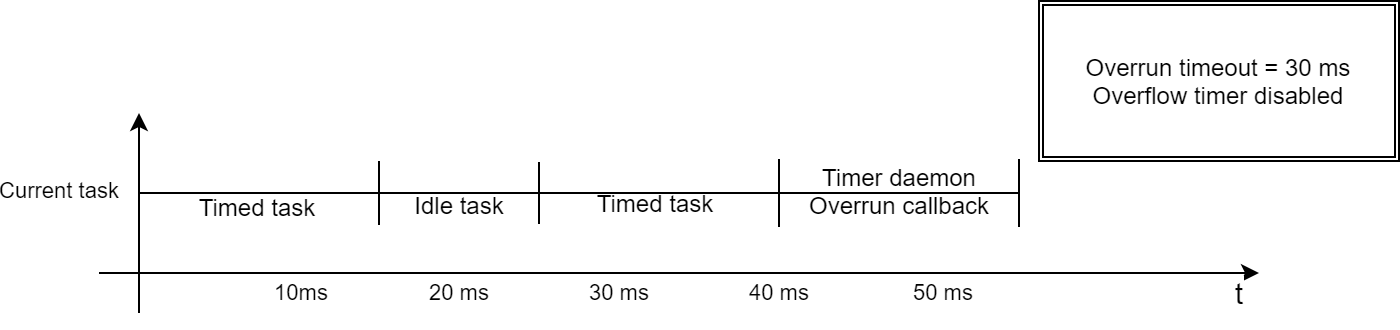
\includegraphics[width=\linewidth]{images/timed_example_overrun.png}
      \caption{Timed task with overrun timeout of 30 ms}
      \label{fig:timed_example_overrun}
    
\end{figure}

\begin{figure}[H]

      \centering
      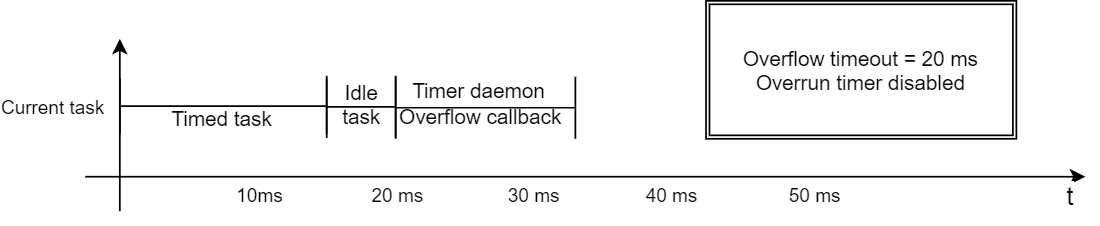
\includegraphics[width=\linewidth]{images/timed_example_overflow.png}
      \caption{Timed task with overflow timeout of 20 ms}
      \label{fig:timed_example_overflow}
    
\end{figure}

\begin{figure}[H]

      \centering
      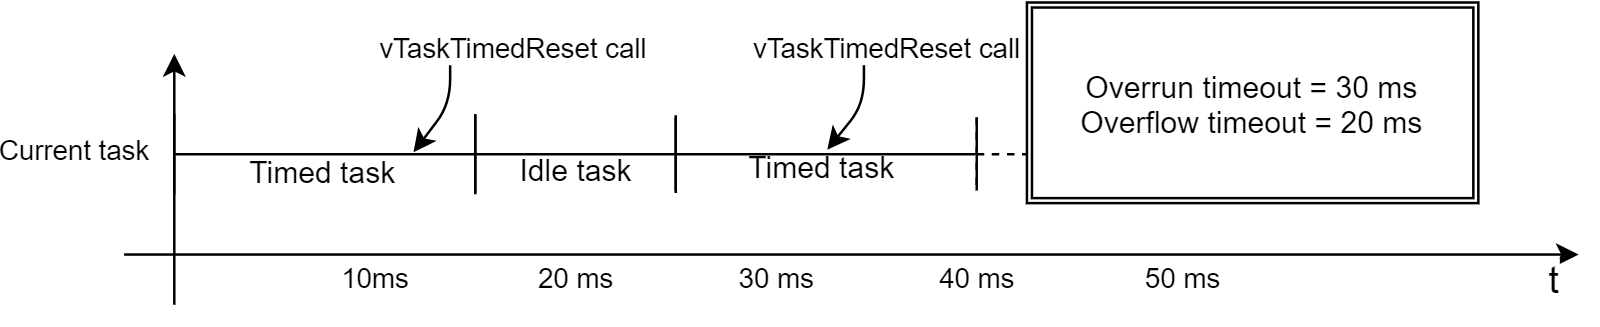
\includegraphics[width=\linewidth]{images/timed_example_reset.png}
      \caption{Timed task with both timers that resets in time}
      \label{fig:timed_example_reset}
    
\end{figure}

Timer callback functions are called by the timer daemon and its priority determines when the callback will be called. It is recommended that the timer daemon has the highest priority. \code{vTaskDelete} function is changed so that deleting tasks also deletes their timers. 

\section{Replicated tasks}

\subsection{Introduction}

Redundancy is a common term with safety hardware, but the redundancy can be achieved with the software. As is demonstrated with the replicated tasks. As the name suggests, when replicated tasks are created they make more parallel instances and they compare outputs of each other to assure no errors happened. 

Hardware redundancy has the advantage of detecting the fault as early as possible at the cost of increased hardware. On the other hand, software redundancy is useful when the system cost is the restriction as no additional hardware is needed. 

\noindent Two types of replicated tasks are implemented:
\begin{itemize}
    \item 2oo2\footnote{MooN is read as M out of N. It shows how many valid outputs have to be present for valid operation e.g. 1oo2 means 1 valid output out of 2 have to be present for a valid operation} configuration or without recovery
    \item 2oo3 configuration or with recovery
\end{itemize}

Recovery of 2oo3 configuration can be achieved with voting logic. Voting logic can determine which two tasks have the same output and make it a valid one. The same is not possible with 2oo2 voting logic. \autoref{appendix_cmd_ref_freertos} contains the command reference for the replicated tasks.

\subsection{Architecture}

Replicated tasks can detect errors using at least two tasks performing identical operations. Tasks are independently processed by the processor. Output variables from tasks are compared in real-time. In case of a discrepancy in the output variables, an error callback is called where the user can process the error.

\autoref{fig:replicated_example} shows how replicated tasks with recovery work. It shows that all instances wait on the barrier. When all tasks have arrived their compare values are compared. In case of a mismatch, the callback given on task creation is called. 


\begin{figure}[H]

      \centering
      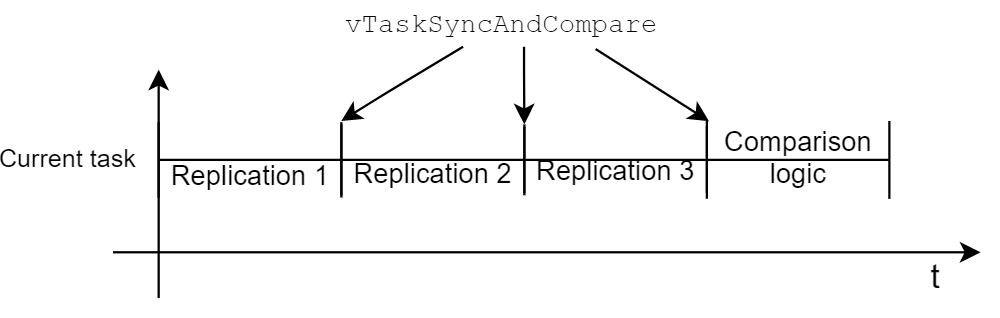
\includegraphics[width=\linewidth]{images/replicated_example.png}
      \caption{Replicated task with redundancy}
      \label{fig:replicated_example}
    
\end{figure}

Comparison logic is not a new task for itself. It is done within one of the tasks, whichever arrives last. \code{vTaskDelete} function was modified so that when one of the replicated sub-tasks delete is requested all linked will be deleted. Tasks are linked over the TCBs\footnote{TCB - Task control block}.


